\documentclass[UTF8,11pt,oneside,fontset=fandol]{ctexbook}
\usepackage[a4paper,margin=25mm,headheight=15pt]{geometry}
\usepackage{amsmath,amssymb,amsthm,mathtools,bm}
\usepackage{booktabs,longtable,array,xcolor,tikz,fancyhdr,graphicx}
\usetikzlibrary{arrows.meta,positioning,calc}
\definecolor{ink}{HTML}{17324D}
\definecolor{blue}{HTML}{166C9D}
\definecolor{brown}{HTML}{A46935}
\usepackage[colorlinks=true,linkcolor=blue,urlcolor=blue,bookmarksnumbered=true,hypertexnames=false]{hyperref}
\usepackage{bookmark}
\hypersetup{pdftitle={3Blue1Brown 中文导学教材：从直觉到证明},pdfauthor={VitaeL04213}}
\setlength{\parskip}{0.35em}
\setlength{\parindent}{2em}
\setlength{\emergencystretch}{3em}
\pagestyle{fancy}
\fancyhf{}
\fancyhead[L]{\small 3Blue1Brown 中文导学教材}
\fancyhead[R]{\small\nouppercase{\leftmark}}
\fancyfoot[C]{\thepage}
\renewcommand{\headrulewidth}{0.3pt}
\newcommand{\R}{\mathbb R}
\newcommand{\C}{\mathbb C}
\newcommand{\dd}{\,\mathrm d}
\newcommand{\e}{\mathrm e}
\newcommand{\ii}{\mathrm i}
\newcommand{\lesson}[3]{\section{#2}\label{lesson:#1}
  {\small\noindent\href{https://www.3blue1brown.com/lessons/#1/}{官方课程：\nolinkurl{#1}}\par}
  \def\currentlean{#3}
  \input{guides/#1}
  \input{intuition/#1}
  \input{media/#1}}
\newcommand{\idea}{\subsection*{要点回看}\paragraph{核心概念}}
\newcommand{\mathpart}{\paragraph{整理成数学语言}}
\newcommand{\examplepart}{\paragraph{完整算例}}
\newcommand{\pitfall}{\paragraph{易错点}}
\newcommand{\exercise}{\paragraph{自测与答案}}
\newcommand{\leanpart}[1]{\paragraph{Lean 对照}{\small\expandafter\nolinkurl\expandafter{\currentlean}}\par #1}
\newcommand{\nextlesson}{\par\medskip}
\newcommand{\chapterreview}[1]{\par\noindent\begin{minipage}{\linewidth}\input{reviews/#1}\end{minipage}\par}
\begin{document}
\begin{titlepage}
\color{ink}
\vspace*{16mm}
{\Large 数学直觉\quad $\longrightarrow$\quad 严格命题\quad $\longrightarrow$\quad 机器校验\par}
\vspace{17mm}
{\Huge\bfseries 3Blue1Brown\par}
\vspace{5mm}
{\Huge\bfseries 中文导学教材\par}
\vspace{8mm}
{\LARGE 引导论述 $\cdot$ 动画实验 $\cdot$ Lean 4\par}
\vspace{15mm}
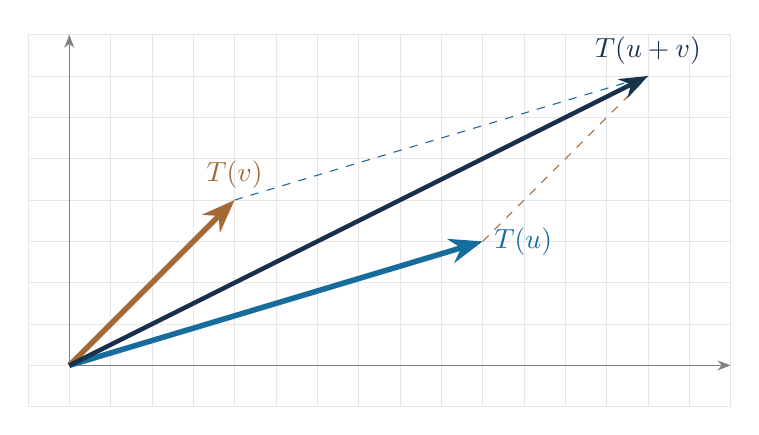
\begin{tikzpicture}[scale=1.05,>=Stealth]
  \draw[step=0.5,gray!20,very thin] (-0.5,-0.5) grid (8,4);
  \draw[->,gray] (0,0)--(8,0);
  \draw[->,gray] (0,0)--(0,4);
  \draw[->,line width=2pt,blue] (0,0)--(5,1.5) node[right] {$T(u)$};
  \draw[->,line width=2pt,brown] (0,0)--(2,2) node[above] {$T(v)$};
  \draw[dashed,blue] (2,2)--(7,3.5);
  \draw[dashed,brown] (5,1.5)--(7,3.5);
  \draw[->,line width=1.6pt,ink] (0,0)--(7,3.5) node[above] {$T(u+v)$};
\end{tikzpicture}
\vfill
{\large 6 组课程\quad 66 个条目\quad 从直觉到推导与验证\par}
\vspace{6mm}
{\large 目录快照：2026 年 10 月 24 日\par}
{\normalsize 独立学习笔记；非 3Blue1Brown 官方出版物。\par}
\end{titlepage}
\frontmatter
\chapter{阅读说明}
\begingroup\small
每节先提出一个具体问题，再用连续论述解释为什么引入概念、怎样选择表示、如何逐步得到公式。正文之后的要点回看、算例与自测用于整理和检查理解。建议先遮住答案独立预测，再观看动画或改变实验参数，最后核对 Lean 命题中的假设；不要让观看替代推导。

配套网页提供原课链接、61 个原视频播放器、9 组原创 Manim 动画和18 类可操作实验。66 节各增加三段逐步讲解，共198段；宽屏页面左侧阅读、右侧操作，每一步可直接复位到对应演示情形。另5个目录条目未单列视频，直接链接官方图文与图示。PDF 共用逐步讲解与18组新增的定义、命题和纸笔证明，放入动画关键帧以及各课的原课、网页和实验入口；静态 PDF 不直接播放动画。网页地址：\url{https://vitael04213.github.io/3blue1brown-notes/}。观课提示定位应关注的概念；未核实的时间点不作标注。

本书按官网五个课程型主题目录整理：线性代数、微积分、神经网络、微分方程及 Lockdown Math；另外纳入有明确集数的“压缩与智能”两集。官网把补充视频也放入这些目录，因此包含散度与旋度、拉普拉斯变换、扩散模型等扩展课。交叉熵同时属于两组，只写一次正文，并在另一处交叉引用。公告页作为学习导读计入，不人为编造数学定理。

范围为该日期已经公开的上述课程序列，共 67 个目录位置、66 节独立课。未把官网“全部”中的每一个独立专题、演讲或外部频道视频算作课程，也不包含未来更新。逐条英文题名、发布日期、原课和视频链接见仓库的 \path{sources/catalog.json} 与 \path{COURSES.md}。

这些内容是围绕课程主题重新组织的中文伴读笔记，含原创计算例与练习，不是字幕全文翻译。对于官网提供正文的课程，参照其概念组织；对于只有标题、简介和视频入口的页面，依据已核实的主题独立推导标准数学内容。没有声称逐帧看完视频。页面获取记录见 \path{sources/retrieval.json}。公式中的实数是精确实数，数值近似会显式使用 $\approx$。

\section*{怎样理解 Lean 校验}
每节末尾列出一个可在仓库中查找的 Lean 定理，并明确校验边界。函数可导、分母非零、概率为正、积分存在等条件会写进定理签名。命名空间统一加前缀 \path{ThreeBlueOneBrown}；例如 \path{Calculus.power_rule} 位于 \path{ThreeBlueOneBrown/Calculus.lean}。

有些 Lean 结果直接复用 mathlib 中已经证明的一般定理，有些是本书的坐标推导或具体例子。通过编译的含义是这些形式命题在 Lean 与 mathlib 的基础下成立；它不意味着视频的一切解释、统计经验或未形式化的分析结论都已经验证。没有使用 \texttt{sorry}、\texttt{admit}、自设公理或 \texttt{native\_decide}。精确的形式化覆盖表见 \path{FORMALIZATION.md}。

先修路线：基础数学，然后线性代数与微积分，再读神经网络和微分方程；信息论适合在概率基础之后阅读。
\endgroup
\tableofcontents
\mainmatter
\chapter{线性代数：把矩阵看成动作}
本章固定列向量约定：$Av$ 表示先给定向量 $v$，再作用矩阵 $A$；$ABv$ 中 $B$ 先作用。几何图像帮助发现结论，坐标与线性映射负责精确定义。

\lesson{vectors}{向量究竟是什么}{LinearAlgebra.vectors_distribute}
\idea 向量可以看成位移、按顺序排列的特征，或满足加法与数乘规则的对象。坐标依赖基的选择，而向量本身不必依赖某一组坐标。
\mathpart 在 $\R^2$ 中，$(x,y)+(u,v)=(x+u,y+v)$，$a(x,y)=(ax,ay)$。数乘对加法分配：$a(u+v)=au+av$，这保证“先合并再缩放”和“先缩放再合并”一致。
\examplepart 取 $u=(2,-1),v=(-1,3)$，则 $u+v=(1,2)$，$2(u+v)=(2,4)=2u+2v$。箭头首尾相接给出同一个结果。
\pitfall 点的位置与位移不是同一个概念；讨论位置向量时已经选了原点。列坐标的顺序也不能交换。
\exercise 求 $3(1,-2)-2(-1,1)$。答案为 $(5,-8)$；交换数乘与相减顺序不会改变结果。
\leanpart{在实数对上完整验证数乘分配律；没有把几何直觉替代成浮点数计算。}
\nextlesson

\lesson{span}{线性组合、张成与基}{LinearAlgebra.coordinates_span}
\idea 张成空间是“给定方向通过任意拉伸、相加能到达哪里”。基要求既能到达整个空间，又没有多余方向。
\mathpart $\operatorname{span}(u,v)=\{au+bv:a,b\in\R\}$。标准基 $e_1=(1,0),e_2=(0,1)$ 满足 $x e_1+y e_2=(x,y)$。若 $u,v$ 不共线，表达式 $au+bv$ 的系数唯一。
\examplepart 对 $u=(1,1),v=(1,-1)$，解 $a+b=4,a-b=2$ 得 $(4,2)=3u+v$。若把 $v$ 换成 $2u$，只能得到直线 $y=x$。
\pitfall “有两个向量”不等于“有二维基”；零向量或共线向量不会增加维数。
\exercise $(3,5)$ 在上述 $u,v$ 基下的坐标是什么？答案 $(4,-1)$，代回为 $(4,4)+(-1,1)$。
\leanpart{验证标准基的张成等式。一般基的线性无关性与坐标唯一性在本节纸笔解释中给出，未在此命题中形式化。}
\nextlesson

\lesson{linear-transformations}{线性变换与矩阵}{LinearAlgebra.linear_combination}
\idea 线性变换保持向量相加与缩放。平面上的网格可以被拉伸、剪切或压扁，但原点固定，平行的直线仍保持平行或塌缩。
\mathpart $T(au+bv)=aT(u)+bT(v)$。矩阵的第 $j$ 列就是 $T(e_j)$，所以
\[A=\begin{bmatrix}2&1\\0&3\end{bmatrix}\quad\Longrightarrow\quad A(x,y)=(2x+y,3y).\]
\examplepart $A(1,2)=(4,6)$，也等于 $T(e_1)+2T(e_2)=(2,0)+2(1,3)$。这从基向量图像直接导出矩阵乘法。
\pitfall 平移 $v\mapsto v+b$ 在 $b\ne0$ 时不是线性变换；它是仿射变换。
\exercise $T(x,y)=(x,y+x^2)$ 是否线性？不是，例如 $T(2,0)=(2,4)\ne2T(1,0)$。
\leanpart{对任意实向量空间间的线性映射验证线性组合保持律，形式化范围比二维例子更广。}
\nextlesson

\lesson{matrix-multiplication}{矩阵乘法就是复合}{LinearAlgebra.matrix_composition}
\idea 矩阵乘法的列，是后一动作的基向量像经过前一动作后的结果。因此乘法次序有实际意义。
\mathpart $(AB)v=A(Bv)$，且 $(AB)_{ij}=\sum_k A_{ik}B_{kj}$。令
\[A=\begin{bmatrix}1&1\\0&1\end{bmatrix},\quad B=\begin{bmatrix}2&0\\0&1\end{bmatrix};\quad
AB=\begin{bmatrix}2&1\\0&1\end{bmatrix},\quad BA=\begin{bmatrix}2&2\\0&1\end{bmatrix}.\]
\examplepart 对 $v=(0,1)$，先 $B$ 后 $A$ 得 $(1,1)$，反过来得到 $(2,1)$。这是不交换性的直接见证。
\pitfall $AB$ 的右边先做；“每个位置对应相乘”是逐元素乘法，不是线性变换复合。
\exercise 为什么 $(AB)C=A(BC)$？两边都对向量执行 $C$、$B$、$A$，或展开有限求和验证。
\leanpart{复用 mathlib 的矩阵作用复合定理，在任意实 $2\times2$ 矩阵和向量上验证等式。}
\nextlesson

\lesson{3d-transformations}{三维线性变换}{LinearAlgebra.rotation_preserves_square_norm}
\idea 三维矩阵有三列，分别记录三个基向量去向。二维的“面积”将在三维变成“体积”。
\mathpart 绕 $z$ 轴逆时针旋转 $90^\circ$ 的矩阵为
\[R=\begin{bmatrix}0&-1&0\\1&0&0\\0&0&1\end{bmatrix},\quad R(x,y,z)=(-y,x,z).\]
\examplepart $(2,1,3)$ 变为 $(-1,2,3)$。两者平方长度均为 $14$，且 $z$ 坐标保持不变；连续作用四次回到原向量。
\pitfall 三维旋转通常不交换；绕不同轴的两个旋转要按顺序处理。
\exercise 对 $(1,0,0)$ 连续作用两次 $R$。答案 $(-1,0,0)$，不是原向量。
\leanpart{验证该 $90^\circ$ 旋转保持平方长度。未宣称已经证明一般三维旋转的分类。}
\nextlesson

\lesson{determinant}{行列式：有向体积倍率}{LinearAlgebra.determinant_product}
\idea 行列式记录面积或体积缩放，同时用符号记录定向是否翻转。压成更低维时，体积归零。
\mathpart 对 $A=\left[\begin{smallmatrix}a&b\\c&d\end{smallmatrix}\right]$，$\det A=ad-bc$。复合的倍率相乘：$\det(AB)=\det A\det B$。
\examplepart 剪切 $S=\left[\begin{smallmatrix}1&3\\0&1\end{smallmatrix}\right]$ 把单位方形推斜，面积仍为 $1$。反射 $F=\operatorname{diag}(-1,1)$ 的行列式为 $-1$，面积大小不变但方向反转。
\pitfall 行列式为负不表示几何面积为负；普通面积倍率是 $|\det A|$。非方阵没有这种同维体积行列式。
\exercise $A=\left[\begin{smallmatrix}2&1\\1&3\end{smallmatrix}\right]$ 的面积倍率？答案 $5$；$A^2$ 为 $25$。
\leanpart{通过坐标展开严格证明两个一般实 $2\times2$ 矩阵的行列式乘法公式。}
\nextlesson

\lesson{inverse-matrices}{逆矩阵、列空间与零空间}{LinearAlgebra.kernel_translation}
\idea $Ax=b$ 是寻找能被送到 $b$ 的输入。列空间描述可到达的输出，零空间描述被压成零的方向。
\mathpart 若 $x_0$ 是一个解，则所有解为 $x_0+\ker A$。方阵可逆当且仅当其零空间只有零向量，也等价于行列式非零。
\examplepart $A=\left[\begin{smallmatrix}1&1\\2&2\end{smallmatrix}\right]$ 的列空间为 $\operatorname{span}(1,2)$，零空间为 $\operatorname{span}(1,-1)$。$Ax=(3,6)$ 的解是 $(3,0)+t(1,-1)$；右端若为 $(3,7)$ 则无解。
\pitfall “不能求逆”不等于“没有解”，也可能有无穷多个解。
\exercise 可逆矩阵的两个不同输入能有同一输出吗？不能；相减后得到一个非零零空间向量，与可逆性矛盾。
\leanpart{证明给任意输入加上核中的向量不会改变输出；形式化的是解集结构的核心方向。}
\nextlesson

\lesson{nonsquare-matrices}{非方阵与维度变化}{LinearAlgebra.projection_surjective}
\idea $m\times n$ 矩阵把 $n$ 维输入映到 $m$ 维输出。行数与列数分别对应输出和输入维度。
\mathpart
\[P=\begin{bmatrix}1&0&0\\0&1&0\end{bmatrix},\quad P(x,y,z)=(x,y),\quad
\ker P=\{(0,0,z):z\in\R\}.\]
它满射但不单射。相反，$J(x,y)=(x,y,0)$ 单射但不是到整个 $\R^3$ 的满射，且 $PJ=I_2$。
\examplepart $(2,5,7)$ 和 $(2,5,-1)$ 都被投到 $(2,5)$。丢失的 $z$ 信息无法从输出恢复。
\pitfall 有左逆或右逆并不一定同时有双侧逆；矩阵形状先于运算公式。
\exercise $JP$ 是什么？它把 $(x,y,z)$ 变为 $(x,y,0)$，不是 $I_3$。
\leanpart{完整证明这一坐标投影满射，构造每个输出 $(x,y)$ 的原像 $(x,y,0)$。}
\nextlesson

\lesson{dot-products}{点积与对偶}{LinearAlgebra.dot_linear}
\idea 固定一个向量 $u$，点积 $v\mapsto u\cdot v$ 就是一个线性测量。几何上它把 $v$ 沿 $u$ 的投影长度乘以 $\|u\|$。
\mathpart $u\cdot v=\sum_i u_iv_i=\|u\|\|v\|\cos\theta$。对 $u\ne0$，投影为 $\operatorname{proj}_u v=\frac{u\cdot v}{u\cdot u}u$。
\examplepart $u=(1,2),v=(3,1)$ 的点积为 $5$，所以投影恰为 $(1,2)$，残差 $(2,-1)$ 与 $u$ 正交。
\pitfall 点积的坐标求和式默认标准正交基。一般基下需使用 Gram 矩阵 $G$，得到 $[u]^T G[v]$。
\exercise 写出线性测量 $L(x,y)=4x-y$ 对应的向量。标准内积下答案 $(4,-1)$。
\leanpart{验证二维点积对第二个输入可加，即固定向量所定义测量的线性结构之一。}
\nextlesson

\lesson{cross-products}{叉积与有向面积}{LinearAlgebra.cross_orthogonal}
\idea 在定向三维欧氏空间中，叉积垂直于两个输入向量；长度等于它们张成的平行四边形面积，方向由右手规则决定。
\mathpart
\[(a,b,c)\times(x,y,z)=(bz-cy,cx-az,ay-bx).\]
从坐标展开可得 $u\cdot(u\times v)=0$；交换顺序改变符号。
\examplepart $(1,2,0)\times(0,1,3)=(6,-3,1)$。与第一个向量点积为 $6-6=0$，与第二个点积也为 $-3+3=0$。
\pitfall 叉积不同于点积：一个输出向量，一个输出标量。其熟悉的三维形式需要内积和定向。
\exercise $(1,0,0)\times(0,1,0)$ 是什么？答案 $(0,0,1)$；反过来为 $(0,0,-1)$。
\leanpart{完整验证一般三维实坐标下，叉积与第一个输入正交。}
\nextlesson

\lesson{cross-products-extended}{从线性测量重新认识叉积}{LinearAlgebra.scalar_triple_product}
\idea 固定 $u,v$，把第三个向量 $w$ 送到有向体积的运算是线性的。这个线性测量可由唯一向量点积表示，而该向量就是 $u\times v$。
\mathpart 对以 $u,v,w$ 为列的矩阵，$\det[u\ v\ w]=(u\times v)\cdot w$。这个标量三重积连接线性代数中的对偶、行列式与几何体积。
\examplepart $u=(1,0,0),v=(0,2,0),w=(a,b,3)$，三重积为 $6$，与 $a,b$ 无关：平行于底面的剪切不改变体积。
\pitfall 行向量和列向量约定混用会造成符号错误；交换任意两列会使有向体积反号。
\exercise 若 $w=u+v$，体积是多少？为零，因为三个向量共面，也可由叉积正交性算出。
\leanpart{展开并验证一般实坐标下的标量三重积等式；唯一表示的抽象论证未包含在该命题中。}
\nextlesson

\lesson{cramers-rule}{克拉默法则}{LinearAlgebra.cramers_rule}
\idea 若矩阵可逆，把一列替换为目标向量，新的有向体积与原体积之比就是相应的坐标系数。
\mathpart 对 $ax+by=p,cx+dy=q$，在 $\Delta=ad-bc\ne0$ 时，
\[x=\frac{pd-bq}{\Delta},\qquad y=\frac{aq-pc}{\Delta}.\]
\examplepart $2x+y=5,x+3y=5$ 给出 $\Delta=5$，故 $x=2,y=1$。几何上新列体积分别为 $10$ 和 $5$。
\pitfall $\Delta=0$ 时不能除以它；此时应改用秩、相容性或零空间判断。该公式也不总是大型数值求解的高效算法。
\exercise 解 $x+2y=4,3x+y=7$。$\Delta=-5$，答案 $x=2,y=1$。
\leanpart{给定两条线性方程和非零行列式，完整推导这两个商公式。}
\nextlesson

\lesson{change-of-basis}{换基：改变坐标语言}{LinearAlgebra.change_of_basis}
\idea 换基改变的是向量的描述。同一个物理动作在不同坐标系统中有不同矩阵。
\mathpart 若 $P$ 的列为新基在旧基下的坐标，则 $[v]_{\rm old}=P[v]_{\rm new}$，且 $[T]_{\rm new}=P^{-1}[T]_{\rm old}P$。
\examplepart 对交换坐标的映射 $A=\left[\begin{smallmatrix}0&1\\1&0\end{smallmatrix}\right]$，选新基 $(1,1),(1,-1)$，得到对角表示 $\operatorname{diag}(1,-1)$。
\pitfall $P$ 的方向必须先定义清楚；如果定义为旧坐标到新坐标，公式中的逆就会对调。
\exercise 上例的 $(3,1)$ 新坐标是什么？解 $a+b=3,a-b=1$，得 $(2,1)$。
\leanpart{用可逆线性等价验证“换回旧坐标后得到原动作”的恒等式，明确要求坐标变换可逆。}
\nextlesson

\lesson{eigenvalues}{特征向量与特征值}{LinearAlgebra.eigenvector_scaling}
\idea 某些方向经过线性变换后只被缩放而不偏离原直线。这些方向常使反复作用变得容易理解。
\mathpart 特征向量满足 $Av=\lambda v$ 且 $v\ne0$。特征值由 $\det(A-\lambda I)=0$ 决定。若有足够多独立特征向量，可写 $A=PDP^{-1}$，进而 $A^n=PD^nP^{-1}$。
\examplepart $A=\left[\begin{smallmatrix}2&1\\1&2\end{smallmatrix}\right]$ 在 $(1,1)$ 上倍率为 $3$，在 $(1,-1)$ 上倍率为 $1$。
\pitfall 零向量虽满足方程却不是特征向量；实矩阵也可能没有实特征值，例如平面 $90^\circ$ 旋转。
\exercise 上例 $A^4(1,1)$？答案 $(81,81)$，无需展开矩阵乘法。
\leanpart{证明特征方程在向量缩放后仍成立。若要称缩放结果为特征向量，还须另加原向量及缩放系数非零的条件。}
\nextlesson

\lesson{quick-eigen}{快速求二维特征值}{LinearAlgebra.characteristic_centering}
\idea 两个根的平均值由迹的一半决定，偏离平均值的距离由判别式决定。先中心化，再处理平方根，比直接套长公式清楚。
\mathpart 令 $m=(a+d)/2$，则
\[\lambda_{\pm}=m\pm\sqrt{((a-d)/2)^2+bc}.\]
根号内为负时，应在复数域解释。来源是特征多项式配方。
\examplepart $A=\left[\begin{smallmatrix}4&2\\1&3\end{smallmatrix}\right]$，$m=3.5$，根号内 $0.25+2=2.25$，故特征值 $5,2$。和为迹 $7$，积为行列式 $10$。
\pitfall 对角元平均值只是根的中心，通常不是其中一个根。
\exercise $\left[\begin{smallmatrix}0&-1\\1&0\end{smallmatrix}\right]$ 的根？根号内 $-1$，为 $\pm\ii$。
\leanpart{验证配方后的特征多项式恒等式。平方根的取值与实根存在性在正文中单独讨论。}
\nextlesson

\lesson{abstract-vector-spaces}{抽象向量空间}{LinearAlgebra.function_space_distribute}
\idea “向量”不必是箭头。多项式、函数、矩阵都可以成为向量，只要其加法与数乘满足同一组公理。
\mathpart 函数空间采用逐点运算：$(f+g)(x)=f(x)+g(x)$，$(af)(x)=af(x)$。微分算子 $D$ 在可微函数组成的适当空间上满足 $D(af+bg)=aDf+bDg$。
\examplepart 在基 $1,x,x^2$ 下，次数不超过二的多项式的求导矩阵为
\[\begin{bmatrix}0&1&0\\0&0&2\\0&0&0\end{bmatrix}.\]
它把系数 $(c_0,c_1,c_2)$ 送到 $(c_1,2c_2,0)$。
\pitfall 指定对象集合还不够；必须说明运算及封闭性。例如“恰好二次”的多项式相加可能不再恰好二次。
\exercise 常数函数为什么在求导算子的核中？因为其导数恒为零。
\leanpart{验证整个实函数空间的数乘分配律。这里只形式化向量空间操作，未把任意函数都错误地视为可微。}

\chapterreview{linear-algebra}
\chapter{微积分：局部变化与累积}
本章以实变量为主，角度使用弧度。导数是局部线性近似的系数，积分是有向累积；极限把近似推进为精确陈述。

\lesson{essence-of-calculus}{从面积发现微积分}{Calculus.area_derivative}
\idea 把圆切成许多薄圆环，半径 $r$ 处的环面积近似为 $2\pi r\,\Delta r$。将所有圆环加起来，自然得到面积是周长的累积。
\mathpart $A(R)=\int_0^R2\pi r\dd r=\pi R^2$，而 $A'(R)=2\pi R$。一般地，连续 $f$ 的累积函数 $F(x)=\int_a^x f(t)\dd t$ 满足 $F'=f$。
\examplepart 对更简单的 $f(t)=t$，面积函数为 $F(x)=x^2/2$，因此增加小宽度 $h$ 的面积是 $xh+h^2/2$；除以 $h$ 后趋向高度 $x$。
\pitfall 薄圆环“长方形化”是极限近似，不能把有限厚度圆环直接当作精确矩形。
\exercise 半径从 $2$ 增到 $2+h$，圆面积多多少？精确值 $4\pi h+\pi h^2$，一阶近似 $4\pi h$。
\leanpart{完整验证简化面积函数 $x^2/2$ 的导数为 $x$；圆环几何分割未形式化。}
\nextlesson

\lesson{derivatives}{导数的“零除以零”悖论}{Calculus.square_secant}
\idea 瞬时速度不是把两个零相除，而是观察非零时间间隔的平均速度在间隔趋零时的趋势。
\mathpart $f'(x)=\lim_{h\to0,h\ne0}\frac{f(x+h)-f(x)}h$。对 $f(x)=x^2$，
\[\frac{(x+h)^2-x^2}{h}=2x+h\quad(h\ne0),\qquad f'(x)=2x.\]
\examplepart $x=3,h=0.01$ 时割线斜率为 $6.01$，它接近切线斜率 $6$，却并不等于它。
\pitfall 不应在约去 $h$ 之前代入 $h=0$；可导也比连续更强，$|x|$ 在零点连续但不可导。
\exercise $|x|$ 在零点的左右斜率？右边 $1$，左边 $-1$，所以双侧导数不存在。
\leanpart{验证非零步长下的差商恒等式，分母条件显式写为 $h\ne0$。导数极限由下一节的形式化幂法则保证。}
\nextlesson

\lesson{derivatives-power-rule}{幂法则的几何来源}{Calculus.power_rule}
\idea 边长增加 $h$ 时，正方形多出两条窄带和一个小角；小角面积是二阶量。立方体的第一阶体积变化来自三个面。
\mathpart 对自然数 $n$，
\[(x+h)^n=x^n+nx^{n-1}h+O(h^2),\qquad (x^n)'=nx^{n-1}.\]
这里的余项表述对固定 $x$、有限多项式成立。实数非整数幂需要额外的定义域条件。
\examplepart $x^3$ 的变化为 $3x^2h+3xh^2+h^3$。差商去极限得到 $3x^2$，在 $x=2$ 处为 $12$。
\pitfall “高阶项很小”必须相对于 $h$ 比较；常数 $n=0$ 的导数为零。
\exercise 求 $f(x)=5x^4-2x^2+7$ 的导数。答案 $20x^3-4x$。
\leanpart{完整调用并验证自然数幂的一般导数定理；Lean 中自然数的 $n-1$ 是截断减法，$n=0$ 由前面的零系数正确处理。}
\nextlesson

\lesson{derivatives-trig-functions}{三角函数的导数}{Calculus.sine_derivative}
\idea 单位圆上匀速运动的切向量，把位置向量旋转 $90^\circ$。因此横坐标 $\cos\theta$ 的速度是 $-\sin\theta$，纵坐标 $\sin\theta$ 的速度是 $\cos\theta$。
\mathpart
\[(\sin x)'=\cos x,\qquad (\cos x)'=-\sin x.\]
弧度让单位圆上的角度增量等于弧长增量，这是导数没有额外比例系数的原因。
\examplepart 在 $x=\pi/3$ 处，正弦高度为 $\sqrt3/2$，变化率为 $1/2$。峰值 $x=\pi/2$ 处的变化率为零。
\pitfall 若输入用“度”，函数其实是 $\sin(\pi x/180)$，导数要乘 $\pi/180$。
\exercise $\sin(2x)$ 的导数是什么？答案 $2\cos(2x)$，需要链式法则。
\leanpart{完整验证实正弦在任意实点的导数；采用 mathlib 的弧度三角函数。}
\nextlesson

\lesson{chain-rule-and-product-rule}{乘积法则与链式法则}{Calculus.chain_rule}
\idea 面积 $fg$ 的增量来自两条边的改变；复合函数的局部伸缩倍率则相乘。
\mathpart
\[(fg)'=f'g+fg',\qquad (g\circ f)'(x)=g'(f(x))f'(x).\]
乘积展开中还有 $\Delta f\Delta g$，可导性保证它除以 $h$ 后趋零。链式法则中的外层导数要在内层输出处求值。
\examplepart $\frac{d}{dx}(x^2\sin x)=2x\sin x+x^2\cos x$；$\frac{d}{dx}\sin(x^2)=2x\cos(x^2)$。
\pitfall 乘积的导数一般不是导数的乘积；把外层求导点写成 $x$ 也常出错。
\exercise $\e^{3x^2}$ 的导数？答案 $6x\e^{3x^2}$。
\leanpart{\texttt{chain\_rule} 与同文件的 \texttt{product\_rule} 完整保留两函数在相应点可导的假设。}
\nextlesson

\lesson{eulers-number}{为什么自然常数 e 特别}{Calculus.exponential_derivative}
\idea 指数增长的变化速度与当前数量成比例。当这个比例常数为 $1$ 时，对应的底数就是 $\e$。
\mathpart $\frac{d}{dx}\e^x=\e^x$，且对 $a>0$，$a^x=\e^{x\ln a}$，所以 $(a^x)'=a^x\ln a$。
\examplepart 连续增长模型 $N(t)=N_0\e^{rt}$ 满足 $N'=rN$。当 $r=\ln2$ 且时间单位为一时，$N(1)=2N_0$。
\pitfall 增长率 $r$ 的单位是时间的倒数；“每年增长 $100\%$”的离散模型与 $r=1$ 的连续模型不同。
\exercise $2^x$ 在零点的斜率？答案 $\ln2$，不是 $1$。
\leanpart{完整验证实指数在每个实点的导数；增长模型只作为数学例子。}
\nextlesson

\lesson{implicit-differentiation}{隐函数求导}{Calculus.circle_tangent}
\idea 曲线由关系式定义，不必先显式解出 $y$。沿曲线移动时，定义关系的总变化必须为零。
\mathpart 若 $F(x,y(x))=0$ 且相关函数可微，则 $F_x+F_y y'=0$。对 $x^2+y^2=1$，当 $y\ne0$ 时 $y'=-x/y$。
\examplepart 在 $(3/5,4/5)$ 处，切线斜率为 $-3/4$，切线方程为 $3x+4y=5$。
\pitfall 圆不全局定义单值 $y(x)$；在 $(\pm1,0)$ 处上述商不能使用，切线垂直。
\exercise 在同一点沿切线有 $dx=0.04$，一阶估计 $dy$。答案 $-0.03$。
\leanpart{从微分约束 $2x\,dx+2y\,dy=0$ 和 $y\ne0$ 推导 $dy=-x\,dx/y$；隐函数存在性定理未形式化。}
\nextlesson

\lesson{limits}{极限与导数的定义}{Calculus.square_limit}
\idea 极限描述输入接近某处时输出是否能被控制到任意精度，并不要求函数在该点已有定义。
\mathpart 连续性是 $\lim_{x\to a}f(x)=f(a)$；导数是另一函数“差商”的去心极限。多项式连续，所以 $\lim_{x\to a}x^2=a^2$。
\examplepart $(x^2-1)/(x-1)$ 在 $x=1$ 未定义，但对 $x\ne1$ 等于 $x+1$，因此极限为 $2$，可用补值修复连续性。
\pitfall 极限存在并不意味着原函数在该点连续；左右极限也可能不同。
\exercise 把上例在 $x=1$ 处定义成 $7$，极限变了吗？没有，仍为 $2$，但不连续。
\leanpart{完整验证平方函数的双侧极限；使用邻域过滤器表达“趋近”。}
\nextlesson

\lesson{epsilon-delta}{把任意精度写清楚}{Calculus.epsilon_delta_linear}
\idea 对方先指定输出容忍误差 $\varepsilon$，我们再给输入误差上限 $\delta$。顺序不能反过来，也不能让 $\delta$ 随后来选择的 $x$ 改变。
\mathpart
\[\forall\varepsilon>0\ \exists\delta>0\ \forall x,
\quad 0<|x-a|<\delta\Rightarrow |f(x)-L|<\varepsilon.\]
\examplepart 对 $f(x)=3x+2,L=3a+2$，选择 $\delta=\varepsilon/3$，因为输出误差恰为 $3|x-a|$。
\pitfall 证明极限不能只代几个小步长。对于平方函数，$|x^2-a^2|=|x-a||x+a|$ 还需要控制第二个因子。
\exercise 若 $f(x)=5x-1$，可取怎样的 $\delta$？取 $\varepsilon/5$ 即可。
\leanpart{显式构造并验证斜率 $3$ 的函数的 $\varepsilon$--$\delta$ 证明；该结论允许 $x=a$，比去心版本更强。}
\nextlesson

\lesson{l-hopitals-rule}{洛必达法则：比较消失速度}{Calculus.removable_limit}
\idea 当分子分母同时趋零时，比值取决于它们接近零的速度。导数可揭示这个速度，但需要足够的可微性条件。
\mathpart 一个常用 $0/0$ 版本要求：$f,g$ 在去心区间可微，$g'\ne0$，$f,g\to0$，且 $f'/g'\to L$；在相应单侧区间条件下可推出 $f/g\to L$。双侧结论须两侧一致。
\examplepart $\lim_{x\to1}(x^2-1)/(x-1)=2$。可以用导数比值 $2x/1$，也可以先因式分解，后者在此更直接。
\pitfall 原比值不是未定式时不能随便求导。例如 $(x+1)/(x+2)$ 在零点的极限为 $1/2$，导数比值却为 $1$。
\exercise 求 $\lim_{x\to0}(\e^x-1)/x$。答案 $1$，由指数函数在零点的导数定义即可得到。
\leanpart{完整验证上述有理函数的去心极限，方法是局部化简与连续性；没有把它标成一般洛必达法则的形式化证明。}
\nextlesson

\lesson{integration}{积分与微积分基本定理}{Calculus.fundamental_theorem}
\idea 积分把每个位置的微小贡献累积起来。如果已知一个变化率的原函数，就能用端点差得到总变化。
\mathpart 若 $F$ 在包含区间的范围内可导且 $F'$ 在区间可积，则
\[\int_a^b F'(x)\dd x=F(b)-F(a).\]
连续被积函数的原函数可由累积积分构造，这是基本定理的另一方向。
\examplepart $\int_1^3 2x\dd x=3^2-1^2=8$。把积分上下限交换，结果变成 $-8$。
\pitfall 定积分是有向累积，不总是几何面积；被积函数为负的部分带负号。原函数的常数在端点差中抵消。
\exercise $\int_{-1}^1 x\dd x$？答案 $0$；两侧几何面积之和却是 $1$。
\leanpart{调用完整的基本定理第二部分，保留区间上处处可导及导函数区间可积的精确假设。}
\nextlesson

\lesson{area-and-slope}{面积为什么与斜率相连}{Calculus.triangle_area}
\idea 右边界移动 $h$，新增窄条的高度接近 $f(x)$。窄条面积除以宽度，便接近原图的高度。
\mathpart $F(x+h)-F(x)=\int_x^{x+h}f(t)\dd t$。若 $f$ 在 $x$ 连续，平均高度趋向 $f(x)$，所以 $F'(x)=f(x)$。
\examplepart $f(t)=t$ 时，$F(x)=\int_0^x t\dd t=x^2/2$。在 $x=2$ 的累积面积为 $2$，面积增长速度也为 $2$，两者单位不同。
\pitfall 累积函数的高度与斜率是不同量；其数值偶然相同并无普遍意义。
\exercise 从 $x=2$ 移到 $2+h$ 的精确面积增量？$2h+h^2/2$；一次近似忽略的部分是三角形面积。
\leanpart{完整验证 $\int_0^a x\dd x=a^2/2$，也涵盖有向积分 $a<0$ 的情况。}
\nextlesson

\lesson{higher-order-derivatives}{高阶导数}{Calculus.second_derivative_cubic}
\idea 一阶导数描述变化，二阶导数描述变化率怎样改变。运动中分别对应速度和加速度；函数图像中二阶导数控制局部凹凸。
\mathpart 对 $f(x)=x^3$，$f'=3x^2$，$f''=6x$，$f'''=6$。一般 $f''(a)>0$ 意味着附近斜率正在增加，但不保证 $f'(a)>0$。
\examplepart $f(x)=x^2$ 在 $x=-1$ 处仍在下降，因为 $f'=-2$，同时向上弯曲，因为 $f''=2$。
\pitfall $f''(a)=0$ 不是拐点的充分条件；$x^4$ 在零点二阶导数为零，但凹凸性不变。
\exercise $f(x)=\sin x$ 的四阶导数？答案仍为 $\sin x$，每四次循环。
\leanpart{完整计算三次函数的二阶导数为 $6x$，同时核实中间的一阶导函数。}
\nextlesson

\lesson{taylor-series}{泰勒多项式与余项}{Calculus.cubic_taylor_exact}
\idea 用多项式逐次匹配函数在一点的值、斜率、曲率等信息。匹配更多导数改善局部近似，但不自动保证无限级数等于原函数。
\mathpart
\[T_n(a+h)=\sum_{k=0}^n\frac{f^{(k)}(a)}{k!}h^k.\]
在相应区间有足够连续导数时，拉格朗日余项为 $f^{(n+1)}(\xi)h^{n+1}/(n+1)!$，其中 $\xi$ 位于两端之间。
\examplepart 对 $f(x)=x^3$，$f(a+h)=a^3+3a^2h+3ah^2+h^3$ 是精确等式；在 $a=1,h=0.1$ 得 $1.331$。
\pitfall 无穷可微不等于解析。把 $\e^{-1/x^2}$ 在零点补为零后，其零点泰勒级数恒零，却不等于邻域中的函数。
\exercise $\e^{0.1}$ 的二阶近似？$1+0.1+0.005=1.105$，须用余项界判断精度。
\leanpart{验证三次多项式的精确泰勒恒等式；一般泰勒定理、级数收敛和余项界未纳入这一形式命题。}
\nextlesson

\lesson{taylor-series-geometric-view}{泰勒展开的面积解释}{Calculus.quadratic_error}
\idea 一阶近似对应窄条的矩形面积；若高度也在变化，再加入三角形面积，就出现二阶修正中的 $1/2$。
\mathpart 由 $F'=f$，在足够光滑时
\[F(a+h)-F(a)=f(a)h+\frac12f'(a)h^2+o(h^2).\]
它正是 $F$ 的二阶泰勒式。
\examplepart 取 $F(x)=x^2$，$f(x)=2x$。矩形贡献为 $2ah$，三角形贡献为 $h^2$，且此时余项恰为零。
\pitfall 三角形近似依赖 $f$ 的局部线性性；对一般曲线、有限大 $h$，不能把它当精确面积。
\exercise $F(x)=x^2/2$ 的一次近似误差？精确为 $h^2/2$，不随展开点 $a$ 改变。
\leanpart{精确验证平方函数减去一次近似后等于 $h^2$；这给出二阶修正的可核查例子。}
\nextlesson

\lesson{derivatives-and-transforms}{导数作为局部变换}{Calculus.derivative_composition_scale}
\idea 把函数看成移动数轴上的点。导数说明一点附近的间距被放大多少，以及是否反向；这种看法可自然推广为多变量的线性映射。
\mathpart 可导性也可写作 $f(a+h)=f(a)+f'(a)h+o(h)$。复合的线性部分相乘，正是链式法则。
\examplepart $x\mapsto x^2$ 在 $a=3$ 附近约放大 $6$ 倍，在 $a=-3$ 附近反向并放大 $6$ 倍。在零点导数为零，但函数没有在整个邻域变成常数。
\pitfall 局部倍率为零并不排除高阶变化；导数是某点的一阶信息。
\exercise 先缩放 $b$ 倍，再缩放 $a$ 倍，总倍率？$ab$；若 $a,b$ 均为负，复合保持方向。
\leanpart{完整验证两个线性缩放复合后的导数为 $ab$。一般非线性链式法则另见本章对应定理。}
\nextlesson

\lesson{divergence-and-curl}{散度与旋度}{Calculus.planar_divergence}
\idea 散度衡量微小区域的净流出趋势，旋度衡量局部环流趋势。二者是不同的局部测量。
\mathpart 对平面向量场 $F=(P,Q)$，$\nabla\cdot F=P_x+Q_y$，标量旋度为 $Q_x-P_y$。对于 $F=(ax,by)$，散度为 $a+b$；对于 $F=(-y,x)$，散度为零、旋度为 $2$。
\examplepart 场 $(x,y)$ 让面积按瞬时相对速率 $2$ 膨胀；旋转场 $(-y,x)$ 保持局部面积却产生旋转。
\pitfall 一个点散度为零只意味着局部净流出抵消，不表示场向量为零；旋度为零的全局势函数结论还与区域拓扑有关。
\exercise $F=(2x,-2y)$ 的散度和旋度？均为零，但它仍会拉伸一个方向并压缩另一个方向。
\leanpart{计算对角线性向量场的两个偏方向导数之和；未形式化散度定理或斯托克斯定理。}

\chapterreview{calculus}
\chapter{神经网络：从像素到序列}
本章把计算规则、训练目标和经验解释分开。公式能描述网络如何运算；“学到了怎样的概念”需要实验，不能仅凭结构图断言。

\lesson{neural-networks}{神经网络的基本单元}{NeuralNetworks.affine_composition}
\idea 把输入表示为向量后，每一层先做带偏置的线性组合，再经过非线性函数。参数控制哪些输入影响哪些输出。
\mathpart
\[z^{(\ell)}=W^{(\ell)}a^{(\ell-1)}+b^{(\ell)},\qquad
a^{(\ell)}=\sigma(z^{(\ell)}).\]
例如 $\sigma(z)=1/(1+\e^{-z})$。若输入维度为 $n$、输出为 $m$，权重形状为 $m\times n$，偏置有 $m$ 个分量。
\examplepart 单神经元 $z=2x_1-x_2+1$，输入 $(1,3)$ 时 $z=0$，Sigmoid 输出为 $1/2$。
\pitfall 没有非线性的多层仿射网络仍可合并成一个仿射映射，深度本身不会产生任意复杂决策边界。
\exercise $x\mapsto3(2x+1)-4$ 可合并为什么？$6x-1$；若中间插入 ReLU，一般不能这样整体合并。
\leanpart{精确验证两个标量仿射层的复合公式，说明非线性激活为何重要。}
\nextlesson

\lesson{gradient-descent}{梯度下降如何学习}{NeuralNetworks.quadratic_gradient_step}
\idea 损失把预测误差压缩为一个标量。梯度指出局部增长最快的方向，向反方向走小步可望减少损失。
\mathpart $\theta_{k+1}=\theta_k-\eta\nabla L(\theta_k)$。一阶近似给出 $\Delta L\approx-\eta\|\nabla L\|^2$，但它只在步长足够小时可信。
\examplepart 对 $L(x)=x^2$，更新为 $x_{+}=(1-2\eta)x$。当 $0\le\eta\le1$ 时损失不增；若 $0<\eta<1$ 且 $x\ne0$，严格减小。$\eta=1$ 时只是来回翻号。
\pitfall 深网络的非凸损失一般不保证达到全局最优；训练损失低也不自动等于新数据上表现好。
\exercise $x=3,\eta=0.1$，更新后损失？$x_+=2.4$，损失 $5.76$，原先为 $9$。
\leanpart{完整证明上述一维二次损失在闭区间步长条件下不增加；没有推广为所有网络的收敛保证。}
\nextlesson

\lesson{neural-network-analysis}{检查网络究竟学到了什么}{NeuralNetworks.affine_input_sensitivity}
\idea 隐层激活不必对应人类想象的边缘或笔画。观察权重、输入扰动和分布外样本，才能检验解释是否与实际计算一致。
\mathpart 对仿射层，扰动满足 $\Delta z=W\Delta x$；在欧氏算子范数下 $\|\Delta z\|\le\|W\|\|\Delta x\|$。这是局部敏感性分析的起点。
\examplepart $z=5x+b$，输入增加 $0.02$，激活前的数值增加 $0.1$。偏置不影响这一差值。对于像素图，平移会改变很多输入坐标，普通全连接层并不天然平移不变。
\pitfall Softmax 的最大概率高，并不保证概率校准，也不意味着输入属于训练分布。
\exercise 为什么只检查训练集准确率不够？模型可能记忆训练样本；还需独立测试及扰动检查。
\leanpart{精确验证单输入仿射模型的扰动等式；范数界、校准与泛化的经验主张未形式化。}
\nextlesson

\lesson{backpropagation}{反向传播的直觉}{NeuralNetworks.gradient_accumulation}
\idea 从输出误差倒推每个中间量的责任：一个节点影响损失的每条路径都要计入，路径上的导数相乘，汇合处相加。
\mathpart 若 $L=L_1+L_2$，则 $\partial L/\partial w=\partial L_1/\partial w+\partial L_2/\partial w$。批量损失为平均值时，梯度也必须取平均。
\examplepart 同一个参数 $w$ 出现在 $L(w)=(w-1)^2+(2w)^2$ 中，导数为 $2(w-1)+8w=10w-2$。只沿第一条路径回传会漏掉 $8w$。
\pitfall 反向传播计算梯度；梯度下降使用梯度更新参数，两者是不同步骤。共享参数不能只保留最后一次出现的梯度。
\exercise 上例最小点？解 $10w-2=0$ 得 $w=1/5$，二阶导数 $10>0$。
\leanpart{完整证明两条可导损失分支相加时导数相加，作为共享梯度累积的标量核心。}
\nextlesson

\lesson{backpropagation-calculus}{反向传播的微积分}{NeuralNetworks.squared_loss_weight_gradient}
\idea 将损失拆成短小的可导计算，再用链式法则组合，避免对整个表达式盲目展开。
\mathpart 对 $z=wa+b,a_{\rm out}=\sigma(z),L=(a_{\rm out}-y)^2$，
\[\frac{\partial L}{\partial w}=2(a_{\rm out}-y)\sigma'(z)a.\]
多层网络写作 $\delta^{(\ell)}=((W^{(\ell+1)})^T\delta^{(\ell+1)})\odot\sigma'(z^{(\ell)})$，权重梯度为 $\delta^{(\ell)}(a^{(\ell-1)})^T$。
\examplepart 线性输出时取 $a=2,b=1,y=4,w=1$，预测为 $3$，权重导数为 $2(3-4)2=-4$；减去负梯度使权重上升。
\pitfall 若损失定义为 $\tfrac12(\hat y-y)^2$，公式中的 $2$ 消失；批量、均值、转置约定必须一致。
\exercise 上例偏置导数是多少？$2(3-4)=-2$。
\leanpart{完整证明线性输出的平方损失对权重的导数。非线性层及矩阵反传公式在正文推导，未由此单命题覆盖。}
\nextlesson

\lesson{mini-llm}{语言模型的简明图景}{NeuralNetworks.conditional_product_bounds}
\idea 语言模型为下一个 token 分配条件概率，采样一个结果后把它放回上下文，继续预测。token 可以是词的一部分，不能总当成完整单词。
\mathpart 概率链式分解为
\[P(x_1,\ldots,x_T)=\prod_{t=1}^T P(x_t\mid x_1,\ldots,x_{t-1}).\]
训练中常最小化正确 token 的负对数概率总和；推理中的采样温度改变概率分布的尖锐程度。
\examplepart 两步条件概率分别为 $0.4,0.25$ 时，这条具体序列的联合概率为 $0.1$，不是 $0.65$。
\pitfall 贪心地每次选最大概率 token，不一定得到全局概率最大的完整序列。
\exercise 概率 $0.5,0.2,0.1$ 的三步序列概率？$0.01$，负对数概率将乘积变成和。
\leanpart{验证两个合法概率的乘积仍在 $[0,1]$；完整条件概率的测度论链式法则未形式化。}
\nextlesson

\lesson{gpt}{Transformer 的整体结构}{NeuralNetworks.softmax_shift}
\idea token 先嵌入为向量，再通过注意力与前馈层反复更新，最后映射为词表上的分数。位置信息使顺序能被模型感知。
\mathpart logits $z_i$ 转成概率：$p_i=\e^{z_i}/\sum_j\e^{z_j}$。对全部分数加同一常数 $c$ 不改变概率，因为共同因子 $\e^c$ 会抵消。
\examplepart 两个 logits 为 $(0,\ln3)$，得到概率 $(1/4,3/4)$。把两者都减去 $\ln3$ 后概率相同，这也是数值稳定 Softmax 的依据。
\pitfall embedding 的某个方向可在特定实验中呈现语义关联，但不能把每一维机械地理解成一个固定概念。
\exercise $z=(2,2)$ 的概率？$(1/2,1/2)$；这与 logits 的绝对大小无关。
\leanpart{完整证明双分类 Softmax 的平移不变性。定理使用精确实指数；浮点稳定性仍属于数值实现问题。}
\nextlesson

\lesson{attention}{注意力：按上下文加权信息}{NeuralNetworks.attention_convex}
\idea 查询向量表达“正在寻找什么”，键向量用于匹配，值向量提供被汇总的信息。每个位置根据自身查询选择不同的权重。
\mathpart 以 token 为行：$Q=XW_Q,K=XW_K,V=XW_V$，
\[\operatorname{Attention}(Q,K,V)=\operatorname{softmax}_{\rm row}\!\left(\frac{QK^T}{\sqrt{d_k}}+M\right)V.\]
因果掩码 $M$ 禁止关注未来位置。每一行的有限权重非负且和为 $1$。
\examplepart 两个标量值 $u=2,v=10$，权重 $(0.75,0.25)$ 得输出 $4$，位于 $[2,10]$ 内。
\pitfall 加权平均的凸包约束只适用于单头的值汇总；输出投影、多个头及残差连接之后，最终向量不必仍在原值凸包内。
\exercise 权重 $(0.2,0.8)$ 时结果？$8.4$。查询与键的维数相同，值维数可以不同。
\leanpart{完整证明两标量值的凸组合处在二者之间，保留权重 $0\le w\le1$ 的条件。}
\nextlesson

\lesson{mlp}{前馈层如何表达特征与关联}{NeuralNetworks.mlp_rank_one}
\idea 前馈层可以先检测输入中的某个方向，再沿另一个方向写回信息。这样能帮助理解关联的存储，但真实网络常使用分布式和叠加表示。
\mathpart $\operatorname{MLP}(x)=W_2\sigma(W_1x+b_1)+b_2$。忽略偏置并在激活处于线性区时，单神经元贡献为 $v(k^Tx)$，等于秩至多为一的矩阵 $vk^T$ 作用于 $x$。
\examplepart $k=(1,2),v=(3,-1),x=(2,1)$，检测值为 $4$，写回向量为 $(12,-4)$。
\pitfall 这种构造说明网络“可以如何”表达一个关联，并不证明某个真实模型恰好如此，也不意味着一个神经元只存一个事实。
\exercise 写出上例的 $vk^T$。答案 $\left[\begin{smallmatrix}3&6\\-1&-2\end{smallmatrix}\right]$，行列式为零。
\leanpart{验证二维检测后写回等于相应外积矩阵作用的坐标公式；不是对模型知识存储机制的经验证明。}
\nextlesson

\section*{延伸阅读：与压缩课程共享的交叉熵}
这一课在官网同时出现在神经网络与“压缩与智能”序列。完整笔记、例子、KL 分解及 Lean 对照统一放在第~\ref{lesson:cross-entropy}~节，以免出现两份相互漂移的版本。

\lesson{diffusion-models}{扩散模型：从噪声中逐步恢复}{NeuralNetworks.denoising_reconstruction}
\idea 正向过程逐渐给数据加噪，反向模型学习在噪声水平及条件信息已知时估计噪声或干净数据。文本条件可通过联合表示和注意力影响生成。
\mathpart 常见正向边际为
\[x_t=\sqrt{\bar\alpha_t}\,x_0+\sqrt{1-\bar\alpha_t}\,\varepsilon,
\qquad\varepsilon\sim\mathcal N(0,I).\]
当 $\bar\alpha_t>0$，若噪声估计为 $\hat\varepsilon$，可构造 $\hat x_0=(x_t-\sqrt{1-\bar\alpha_t}\hat\varepsilon)/\sqrt{\bar\alpha_t}$。
\examplepart 用简化标量系数 $a=0.8,b=0.6,x_0=2,\varepsilon=-1$，得到 $x_t=1$；已知真噪声时 $(1-0.6(-1))/0.8=2$。
\pitfall 上述代数恢复要求知道噪声；模型实际只是估计它。单个带噪样本通常不能唯一确定原始图像。
\exercise 若噪声估计多了 $\delta$，恢复误差是什么？$-(b/a)\delta$，说明 $a$ 很小时误差会被放大。
\leanpart{完整验证非零信号系数下的代数恢复式；未形式化随机扩散过程、训练有效性或生成质量。客座原课署名 Stephen Welch。}

\chapterreview{neural-networks}
\chapter{微分方程：从局部规律到整体演化}
微分方程给出状态的变化规则，初始条件选择具体轨迹，边界条件限制空间上的可行行为。一个显式解公式不是理解系统的唯一方式。

\lesson{differential-equations}{微分方程与向量场}{DifferentialEquations.exponential_solution}
\idea 与其先寻找闭式解，不如在每个状态处画出速度。解曲线必须始终沿着这些箭头前进；相空间把位置和速度合并为状态。
\mathpart 一阶系统写成 $x'=F(t,x)$。二阶摆方程 $\theta''=-(g/L)\sin\theta$ 可改写为 $\theta'=\omega,\ \omega'=-(g/L)\sin\theta$。
\examplepart 最简单的 $x'=kx$ 有解 $x(t)=x_0\e^{kt}$。若 $k<0$，它趋近零；若 $k>0$，非零初值的绝对值增大。
\pitfall 画出方向场不自动保证唯一解；存在唯一性定理需要连续性、局部 Lipschitz 等相应条件。欧拉法也只是近似。
\exercise $x'=2x,x(0)=3$ 的解？$3\e^{2t}$，代回可直接检查。
\leanpart{完整验证 $\e^{kt}$ 的导数等于 $k\e^{kt}$；不是对所有微分方程的存在唯一性证明。}
\nextlesson

\lesson{pdes}{偏微分方程与热扩散}{DifferentialEquations.heat_stencil}
\idea 温度同时依赖位置和时间。热从较热处流向较冷处，局部的“比邻居更高还是更低”决定温度怎样变化。
\mathpart 一维均匀介质模型为 $u_t=\kappa u_{xx}$，$\kappa>0$。离散空间中，
\[u_{xx}(x)\approx\frac{u(x-h)-2u(x)+u(x+h)}{h^2}.\]
这个二阶差分是局部平均恢复趋势的代数版本。
\examplepart 邻点温度为 $4,10,6$，中心二阶差分分子为 $-10$，所以中心倾向降温。若为 $6,2,8$，分子为 $10$，中心倾向升温。
\pitfall 需要给初始温度分布及边界条件；固定端温度与绝热边界是不同问题。显式数值时间步也受稳定性限制。
\exercise 为什么两个解相加仍满足齐次热方程？时间导数与空间二阶导数都线性。
\leanpart{验证三点二阶差分算子对相加的线性性；连续 PDE 的分析及离散极限未由此命题覆盖。}
\nextlesson

\lesson{heat-equation}{用基本模式求解热方程}{DifferentialEquations.heat_mode_decay}
\idea 找到形状在扩散中保持、只改变振幅的波形，再将一般初始数据组合成这些模式。高频因弯曲更强而衰减更快。
\mathpart 对 $0<x<L$ 的零温边界，模式为
\[u_n(x,t)=b_n\sin\frac{n\pi x}{L}\,
\exp\!\left[-\kappa\left(\frac{n\pi}{L}\right)^2t\right].\]
因正弦的二阶导数为频率平方的负倍数，代入后两边相等。
\examplepart 取 $L=\pi,\kappa=1$，$u=\sin x\e^{-t}+2\sin(3x)\e^{-9t}$。第三模式的衰减指数是第一模式的九倍。
\pitfall 无限求和与求导交换需要收敛或正则性条件；边界不是零温时需换模式或先减去稳态。
\exercise 初值仅为 $\sin(2x)$，同样参数下解是什么？$\sin(2x)\e^{-4t}$。
\leanpart{完整验证模式振幅的时间导数。空间正弦导数可由微积分模块组合；无限级数解与边界条件未形式化。}
\nextlesson

\lesson{fourier-series}{傅里叶级数：旋转与叠加}{DifferentialEquations.fourier_superposition}
\idea 正弦、余弦可以合并成复平面上的旋转。不同频率的旋转向量相加，能表示复杂的周期变化。
\mathpart 对周期 $T$，令 $\omega_0=2\pi/T$，
\[f(t)\sim\sum_{n\in\mathbb Z}c_n\e^{\ii n\omega_0t},\qquad
c_n=\frac1T\int_0^T f(t)\e^{-\ii n\omega_0t}\dd t.\]
正交性使积分能够挑出对应频率。
\examplepart $f(t)=3+2\cos t$ 的非零复系数为 $c_0=3,c_1=c_{-1}=1$。常数项不转，其余两个方向相反地旋转。
\pitfall 对不连续周期函数，点态收敛需条件；常见分段光滑情形在跳跃点趋向左右极限的平均值，且会出现 Gibbs 振铃。
\exercise $\sin t$ 的复系数？$c_1=1/(2\ii),c_{-1}=-1/(2\ii)$。
\leanpart{验证单频复指数模式的线性叠加恒等式；不将它冒充傅里叶完备性或收敛定理。}
\nextlesson

\lesson{complex-exponents}{复指数与旋转的物理图像}{DifferentialEquations.rotating_exponential_norm}
\idea 乘以 $\ii$ 表示旋转 $90^\circ$。若速度始终是位置旋转后的向量，运动便沿圆周持续进行。
\mathpart $z'=(\sigma+\ii\omega)z$ 的解为 $z(t)=z_0\e^{\sigma t}\e^{\ii\omega t}$。实部 $\sigma$ 控制增长或衰减，虚部 $\omega$ 控制角速度。
\examplepart $z'=(-1+2\ii)z$ 产生向内螺旋：模长按 $\e^{-t}$ 衰减，角度每单位时间增加 $2$ 弧度。
\pitfall 复数在这里把两个实维度的系统压缩为一个表达式，并不引入“虚假的”物理量；测量量常取实部。
\exercise $\e^{3\ii t}$ 的模长和周期？模长 $1$，周期 $2\pi/3$。
\leanpart{完整验证任意实角度的纯旋转复指数模长为一。}
\nextlesson

\lesson{laplace-transform}{拉普拉斯变换：带衰减的频率探测}{DifferentialEquations.laplace_kernel}
\idea 傅里叶核只旋转；拉普拉斯核同时旋转和指数加权。加入衰减可让原本无法绝对积分的函数变得可处理。
\mathpart 单边变换为 $F(s)=\int_0^\infty f(t)\e^{-st}\dd t$，$s=\sigma+\ii\omega$。对实 $a$，
\[\mathcal L\{\e^{at}\}(s)=\frac1{s-a},\qquad \operatorname{Re}s>a.\]
这个条件保证积分在无穷远收敛。
\examplepart $f(t)=\e^{2t}$ 的变换在实 $s=3$ 处为 $1$，在 $s=1$ 处原积分发散，不能仅把形式有理式代进去当作积分值。
\pitfall 代数表达式与收敛域共同构成变换信息；有理式在某点有值不等于定义积分收敛。
\exercise 常数函数 $1$ 的单边变换？$1/s$，要求 $\operatorname{Re}s>0$。
\leanpart{验证实指数与拉普拉斯核相乘后合并为 $\e^{-(s-a)t}$ 的恒等式；不声称该恒等式本身证明了反演定理。}
\nextlesson

\lesson{laplace-for-odes}{把微分方程变成代数方程}{DifferentialEquations.transformed_oscillator}
\idea 积分分部把求导转换为乘 $s$，同时保留初始值。于是线性常系数方程可以在变换域中求解。
\mathpart 在所需光滑、增长及收敛条件下，$\mathcal L(y')=sY-y(0)$，$\mathcal L(y'')=s^2Y-sy(0)-y'(0)$。若 $y''+\omega^2y=f$，则
\[Y(s)=\frac{F(s)+sy_0+v_0}{s^2+\omega^2}.\]
\examplepart $f=0,y_0=0,v_0=1$ 给 $Y=1/(s^2+\omega^2)$，当 $\omega>0$ 时对应 $y(t)=\sin(\omega t)/\omega$。
\pitfall 漏掉初始值项会改变所求解。极点描述模态，但只有结合收敛域与变换约定才能正确反演。
\exercise $y'+2y=0,y(0)=3$ 的变换与解？$Y=3/(s+2)$，$y=3\e^{-2t}$。
\leanpart{从已得到的变换域等式及非零分母推导商公式。积分分部、拉普拉斯存在性和反演不在该形式命题中。}
\nextlesson

\lesson{eulers-formula-dynamically}{动态理解欧拉恒等式}{DifferentialEquations.euler_identity}
\idea 复指数 $\e^{\ii t}$ 从 $1$ 出发沿单位圆运动，走过 $\pi$ 弧度后到达 $-1$。
\mathpart $\e^{\ii t}=\cos t+\ii\sin t$，所以 $\e^{\ii\pi}+1=0$。也可比较两边的微分方程 $z'=\ii z$ 与初始值 $z(0)=1$，在唯一性定理下识别二者。
\examplepart $t=\pi/2$ 时值为 $\ii$，$t=2\pi$ 时回到 $1$。四个四分之一圈的乘积为 $\ii^4=1$。
\pitfall $\e^{z+w}=\e^z\e^w$ 在复数上成立，但取复对数后要考虑分支，不能直接取消周期性。
\exercise $\e^{-\ii\pi}$ 是多少？同样为 $-1$；方向不同，终点相同。
\leanpart{完整验证复指数的欧拉恒等式，复用 mathlib 已证明的结论。}
\nextlesson

\lesson{matrix-exponents}{矩阵指数与线性动力系统}{DifferentialEquations.nilpotent_exponential_add}
\idea 标量指数把“按当前大小增长”变成演化；矩阵指数把“速度由当前向量线性决定”变成多维演化。
\mathpart $\e^{tA}=\sum_{n\ge0}t^nA^n/n!$，线性系统 $x'=Ax$ 的解为 $x(t)=\e^{tA}x_0$。若 $A^2=0$，级数截断为 $I+tA$。
\examplepart $A=\left[\begin{smallmatrix}0&1\\0&0\end{smallmatrix}\right]$ 满足 $A^2=0$，所以 $\e^{tA}=\left[\begin{smallmatrix}1&t\\0&1\end{smallmatrix}\right]$。初值 $(0,2)$ 演化为 $(2t,2)$。
\pitfall 一般 $\e^{A+B}\ne\e^A\e^B$，交换条件至关重要。逐元素取指数也不是矩阵指数。
\exercise 为什么上例先演化 $s$ 再演化 $t$ 等于演化 $s+t$？$(I+sA)(I+tA)=I+(s+t)A$，因为 $A^2=0$。
\leanpart{完整证明平方零矩阵的上述半群恒等式；矩阵指数级数的收敛与求导由正文解释，未包含于此定理。}
\nextlesson

\lesson{exponential-and-epidemics}{指数增长与饱和}{DifferentialEquations.logistic_threshold}
\idea 若增长速度正比于当前数量，就会出现指数增长。资源或易感群体有限时，固定相对增长率通常只适合早期阶段。
\mathpart 指数模型 $N'=rN$ 的倍增时间为 $\ln2/r$（$r>0$）。一个简化饱和模型是 $N'=rN(1-N/K)$，其中 $K>0$；在 $0<N<K$ 时仍增长，但相对增长率逐渐降低。
\examplepart 若相对增长率从 $r$ 降为 $r/2$，在指数近似下倍增时间翻倍。对 Logistic 模型，$N=K/2$ 时增长率为 $rK/4$。
\pitfall 这是数学教学模型；观测数据、报告延迟和行为改变均可能使真实时间序列偏离模型，不能仅凭曲线外形确认机制。
\exercise Logistic 模型的平衡点有哪些？$N=0$ 和 $N=K$；对 $r>0$，区间 $(0,K)$ 内导数为正。
\leanpart{验证正增长率、正容量且状态处于 $(0,K)$ 时导数严格为正；未形式化流行病预测或参数估计。}

\chapterreview{differential-equations}
\chapter{Lockdown Math：重新组织基础数学}
这一组从高中代数、三角函数和复数出发，把看似独立的公式联成一条学习路径。公告是导读，其余十节有数学正文与对应 Lean 结果。

\lesson{lockdown-math-announcement}{课程公告与学习路线}{not-applicable}
\idea 这是一组由基础概念逐步深入的直播课程。学习时可以把“定义”“例子”“猜想”“证明”分别记下；直播中的探索过程不应被压缩成只有结论的公式表。
\mathpart 推荐先掌握二次方程和单位圆，再学复数、复指数与对数，最后处理幂塔和复数幂。每一步都检查新符号的定义域与旧代数规律是否仍成立。
\examplepart 将 $\sqrt{x^2}=x$ 写入笔记前，应代入 $x=-1$。反例提示正确实数恒等式是 $\sqrt{x^2}=|x|$。
\pitfall 看懂讲解不等于能独立重建推导。复习时先遮住答案，画图、做特殊例、检查边界，再写一般论证。
\exercise 用自己的话区分“例子支持猜想”和“证明结论”。答案要点：有限个例子不能穷尽一般情形，但一个反例足以否定全称命题。
\leanpart{不适用：这是公告和学习方法页，没有需要机器证明的课程命题。仓库的覆盖统计对此显式豁免。}
\nextlesson

\lesson{ldm-quadratic}{更简洁的二次公式}{Lockdown.quadratic_centering}
\idea 把两个根看成“中心 $m$ 加减偏移 $d$”，和与积就变为 $2m$ 与 $m^2-d^2$。
\mathpart 对 $x^2-2mx+p=0$，配方得到 $(x-m)^2=m^2-p$，所以 $x=m\pm\sqrt{m^2-p}$。一般二次式须先除以非零二次项系数。
\examplepart $x^2-10x+21=0$，根的中心为 $5$，偏移平方为 $25-21=4$，故根为 $3,7$。
\pitfall 根号内为负时没有实根，但可以有复根；使用中心形式并没有免除域的选择。
\exercise 根的和为 $8$、积为 $12$，求根。中心 $4$，偏移 $2$，答案 $2,6$。
\leanpart{完整验证配方恒等式；从平方等式分类实根或复根需另行处理。}
\nextlesson

\lesson{ldm-trigonometry}{三角函数从单位圆出发}{Lockdown.unit_circle}
\idea 单位圆将角度和坐标联系起来：$\cos\theta$ 是横坐标，$\sin\theta$ 是纵坐标。三角恒等式可由旋转、投影和勾股关系产生。
\mathpart $\sin^2\theta+\cos^2\theta=1$，且旋转矩阵为
\[R_\theta=\begin{bmatrix}\cos\theta&-\sin\theta\\\sin\theta&\cos\theta\end{bmatrix}.\]
$R_\alpha R_\beta=R_{\alpha+\beta}$ 可导出和角公式。
\examplepart 对 $\theta=\pi/3$，坐标为 $(1/2,\sqrt3/2)$，平方和为 $1/4+3/4=1$。
\pitfall $\sin(\alpha+\beta)$ 通常不等于 $\sin\alpha+\sin\beta$。角度单位改变时，涉及导数的公式需相应换算。
\exercise $\cos(\pi-\theta)$ 和 $\sin(\pi-\theta)$？分别为 $-\cos\theta$、$\sin\theta$。
\leanpart{完整验证实数任意角度的单位圆恒等式。}
\nextlesson

\lesson{ldm-complex-numbers}{复数：缩放与旋转}{Lockdown.complex_square_i}
\idea 实数乘法能缩放数轴，复数乘法还能旋转平面。新单位 $\ii$ 满足 $\ii^2=-1$，与二维坐标运算一致。
\mathpart $(a+b\ii)(c+d\ii)=(ac-bd)+(ad+bc)\ii$。若写成极坐标 $r\e^{\ii\theta}$，相乘时模长相乘、角度相加。
\examplepart $(1+\ii)^2=2\ii$：两个 $45^\circ$ 旋转合为 $90^\circ$，模长从 $\sqrt2$ 平方为 $2$。
\pitfall 复数不能像实数那样建立兼容乘法的全序；“更大”必须说明比较模长、实部或其他量。
\exercise $1/(1+\ii)$ 是什么？乘共轭得 $(1-\ii)/2$。
\leanpart{验证复数单位的核心关系 $\ii^2=-1$；其余运算公式可通过复数域的代数规则推出。}
\nextlesson

\lesson{ldm-eulers-formula}{欧拉公式在说什么}{Lockdown.exponential_add}
\idea 指数将加法转换为乘法；纯虚数指数把角度相加转换为旋转复合。这统一了三角恒等式与指数规律。
\mathpart $\e^{\ii\theta}=\cos\theta+\ii\sin\theta$，并且 $\e^{z+w}=\e^z\e^w$。比较实部与虚部便得到和角公式。
\examplepart $\e^{\ii\pi/3}\e^{\ii\pi/6}=\e^{\ii\pi/2}=\ii$；这比逐项展开两个三角表达式更短。
\pitfall 欧拉公式不是把实指数的图像“转过去”就自动成立；可以由幂级数或微分方程严谨建立。
\exercise $\e^{x+\ii y}$ 的模长是多少？$\e^x$，角度在模 $2\pi$ 意义下为 $y$。
\leanpart{完整验证复指数的加法到乘法规则。欧拉特值另由微分方程模块中的 \texttt{euler\_identity} 验证。}
\nextlesson

\lesson{ldm-imaginary-interest}{虚数利率与连续旋转}{Lockdown.imaginary_step_norm}
\idea 把复利每一步的增长率改成纯虚数，每个小步就增加一个切向位移；步长越来越小时，轨迹趋于圆周运动。
\mathpart 离散近似为 $(1+\ii t/n)^n$。单步模长平方为 $1+(t/n)^2$，整个模长为 $(1+t^2/n^2)^{n/2}$，其极限为 $1$。
\examplepart 单步取 $h=0.1$，$1+0.1\ii$ 的模长是 $\sqrt{1.01}>1$；有限步的轨迹略向外扩张，这个误差在连续极限消失。
\pitfall 每一个离散步骤都不是精确旋转；其模长大于一。不能把极限性质反过来当成有限步恒等式。
\exercise $h=1$ 时，乘 $1+\ii$ 后角度和模长怎样变化？增加 $\pi/4$，模长乘 $\sqrt2$。
\leanpart{验证单步复数的模长平方公式。复利序列收敛到复指数的极限定理未在此命题中形式化。}
\nextlesson

\lesson{ldm-logarithms}{对数的基础结构}{Lockdown.logarithm_product}
\idea 对数把乘法关系改写为加法关系。它是指数函数的反函数，因此必须清楚底数和定义域。
\mathpart 对实数 $a,b>0$，$\ln(ab)=\ln a+\ln b$；对底数 $c>0,c\ne1$，$\log_c a=\ln a/\ln c$。
\examplepart $\log_2 8=3$，因为 $2^3=8$。$\log_2(8\cdot4)=3+2=5$，乘法变成指数相加。
\pitfall 实对数不能直接输入负数；$\log(a+b)$ 没有一般的加法拆分式。复对数的乘法公式还受分支影响。
\exercise $\log_3(1/9)$？答案 $-2$。负的是对数值，真数仍为正。
\leanpart{完整验证正实数乘积的自然对数公式，并显式要求两个真数为正。}
\nextlesson

\lesson{ldm-natural-logs}{自然对数为何自然}{Lockdown.natural_log_derivative}
\idea $\ln$ 把相对变化变成加性变化：若 $x$ 小幅增加 $dx$，则 $d\ln x\approx dx/x$。这让相同比例的增长具有相同对数增量。
\mathpart 对 $x>0$，$(\ln x)'=1/x$，且 $\ln x=\int_1^x dt/t$。与 $\e^x$ 互逆给出 $\ln(\e^x)=x$。
\examplepart $x$ 从 $100$ 增为 $101$，对数增量 $\ln1.01\approx0.00995$，一阶估计为 $0.01$。
\pitfall 近似 $\ln(1+h)\approx h$ 只适用于 $h$ 接近零且 $1+h>0$；它不是全局恒等式。
\exercise $\ln(x^2)$ 在 $x>0$ 时的导数？$2/x$；也可先写成 $2\ln x$。
\leanpart{完整验证正实数处的自然对数导数，写明 $x>0$ 避免除零和实定义域误解。}
\nextlesson

\lesson{ldm-power-towers}{幂塔与不动点}{Lockdown.tower_limit_fixed_point}
\idea 无限幂塔应先定义为有限迭代，再讨论其极限。如果迭代确实收敛，极限才必须满足不动点方程。
\mathpart 对 $a>0$，令 $x_0=1,x_{n+1}=a^{x_n}$。若 $x_n\to L$，由连续性得到 $L=a^L$。局部稳定性的常用线性判据是 $|a^L\ln a|=|L\ln a|<1$。
\examplepart $a=\sqrt2$ 时 $L=2$ 和 $L=4$ 都满足方程；在前者的导数为 $\ln2<1$，后者为 $2\ln2>1$。不动点不一定是从给定初值可达的稳定极限。
\pitfall 解出 $L=a^L$ 仅给必要条件，不能用它证明迭代收敛。完整参数范围还需要单调性、有界性等分析。
\exercise $a=1$ 时该迭代的每一项与极限？都为 $1$。
\leanpart{完整证明一般连续迭代在已知收敛时，其极限为不动点；收敛是假设，绝不隐含在代数方程里。}
\nextlesson

\lesson{ldm-i-to-i}{为什么 i 的 i 次方可以是实数}{Lockdown.i_log_branch_exponent}
\idea 复数幂通过复对数定义。复对数记录角度，而角度相差整圈时对应相同复数，因此必须指定分支。
\mathpart $\log\ii=\ii(\pi/2+2\pi k)$，$k\in\mathbb Z$。于是多值解释下
\[\ii^{\ii}=\exp\bigl[-(\pi/2+2\pi k)\bigr].\]
选择主对数时 $k=0$，主值为 $\e^{-\pi/2}\approx0.20788$。
\examplepart 关键代数是 $\ii\cdot(\ii\theta)=-\theta$，使指数变成实数。不同 $k$ 给出不同正实值，而非单个必然唯一的答案。
\pitfall 不指定对数分支就使用 $(z^a)^b=z^{ab}$ 可能出错；该实数幂习惯不能原样推广。
\exercise 主值 $\ii^{2\ii}$ 是多少？$\e^{-\pi}$，使用相同主对数定义。
\leanpart{验证任意实角度的关键指数恒等式 $\ii(\theta\ii)=-\theta$；并未将多值复幂误写成全局单值定理。}
\nextlesson

\lesson{ldm-tips-to-problem-solving}{解题：找表示、找不变量、查边界}{Lockdown.symmetric_problem_reduction}
\idea 遇到困难时可以先做小例子、画图、改变表示，或寻找在变换下不变的量。目标是减少独立信息，而不是堆积运算。
\mathpart 对称表达式常改用和 $s=x+y$ 与积 $p=xy$，因为 $x^2+y^2=s^2-2p$。这种替换也连接到二次方程与矩阵的迹、行列式。
\examplepart 已知 $x+y=7,xy=10$，不必先求 $x,y$，就能得到 $x^2+y^2=49-20=29$。再求根会得到 $2,5$，作为交叉检查。
\pitfall 一种表示简化目标后，还需保留可行性条件。例如实数 $x,y$ 要满足 $s^2-4p\ge0$。
\exercise 已知 $x+y=3,xy=1$，求 $x^3+y^3$。用 $s^3-3ps$ 得 $27-9=18$。
\leanpart{完整验证对称二次式的代数变换。一般解题策略不是数学全称定理，不声称已被形式化证明。}

\chapterreview{lockdown-math}
\chapter{压缩与智能：熵和交叉熵}
官网截至目录快照日公开的这组编号课程有两集。本章先用二进制位解释编码，再用自然对数写 Lean 公式；两种单位只相差常数 $\ln2$。

\lesson{entropy}{熵：平均要问多少个二选一问题}{Information.entropy_term_nonnegative}
\idea 常见事件可以分配短码，罕见事件用长码。编码的平均长度取决于整个概率分布，而不只是符号总数。
\mathpart 对有限分布 $p_i\ge0,\sum_i p_i=1$，Shannon 熵为
\[H_2(p)=-\sum_i p_i\log_2p_i,\qquad 0\log_2 0:=0.\]
理想信息长度为 $-\log_2p_i$。独立同分布源的长块编码能让平均每符号长度逼近熵；单符号前缀码的整数长度通常有额外开销。
\examplepart 分布 $(1/2,1/4,1/4)$ 可用前缀码 $0,10,11$，平均长度为 $\tfrac12\cdot1+\tfrac14\cdot2+\tfrac14\cdot2=1.5$ 位，恰好等于熵。
\pitfall 熵不是某个特定字符串的长度，也不直接等同于人类语义。对有相关性的序列，要用条件熵或熵率，而不能只看单个符号频率。
\exercise 四个等概率符号的熵是多少？$2$ 位；一个概率为 $1$ 的确定符号的熵为零。
\leanpart{验证正概率 $p\le1$ 的单项 $-p\ln p$ 非负。代码还定义了有限分布的熵；编码下界、可达性和熵率并未形式化。}
\nextlesson

\lesson{cross-entropy}{交叉熵：错误概率模型的编码代价}{Information.cross_entropy_decomposition}
\idea 数据真实分布是 $p$，编码或预测使用的模型是 $q$。模型给真实常见事件过小的概率，就会在这些事件上支付更长的编码代价。
\mathpart 在 $p_i,q_i>0$ 时，
\begin{align*}
H(p,q)&=-\sum_i p_i\ln q_i,\\
D_{\rm KL}(p\|q)&=\sum_i p_i\ln\frac{p_i}{q_i},\\
H(p,q)&=H(p)+D_{\rm KL}(p\|q).
\end{align*}
若 $p,q$ 均归一化，则 $D_{\rm KL}\ge0$。用 $\ln u\le u-1$，对 $u=q_i/p_i$ 逐项乘以 $p_i$ 并求和，即可证明该不等式。
\examplepart 真实分布为 $(1/2,1/2)$，模型为 $(3/4,1/4)$。以位为单位，真实熵为 $1$，交叉熵为 $-\tfrac12\log_2(3/4)-\tfrac12\log_2(1/4)\approx1.20752$，多付约 $0.20752$ 位。
\pitfall $D_{\rm KL}(p\|q)$ 一般不对称，不是距离。若 $p_i>0$ 而 $q_i=0$，扩展意义下代价为无穷，不能直接套普通实数对数代数。
\exercise 正确标签是类别 $j$ 时，单样本交叉熵为何为 $-\ln q_j$？因为 one-hot 标签使其余求和系数均为零。$q_j=1$ 时损失为零。
\leanpart{完整验证严格正有限向量的熵、交叉熵与 KL 代数分解；此分解本身不要求归一化。同文件的 \texttt{kl\_nonnegative} 进一步在两分布归一化时证明 KL 非负；零概率与无穷代价情形不在这两个定理的覆盖范围内。}

\chapterreview{compression}
\backmatter
\chapter{来源与复现}
原课程由 Grant Sanderson 及其署名合作者创作；扩散模型客座课程署名 Stephen Welch / Welch Labs。本书未附带原视频、原图、字幕全文或原网站正文。所有示意图均为本项目重绘的数学图形。

\begin{itemize}
\item 官方目录：\url{https://www.3blue1brown.com/}
\item 官方频道：\url{https://www.youtube.com/@3blue1brown}
\item Lean：\url{https://lean-lang.org/}
\item mathlib：\url{https://github.com/leanprover-community/mathlib4}
\end{itemize}
本项目固定 Lean 4.19.0 和 mathlib 的同版本发布提交。构建命令与验证报告见仓库 README；PDF 是相同 LaTeX 源码的构建产物。更新目录时，先比较新增或删除的课程，再逐项补正文和形式化覆盖说明，不能只修改完成计数。
\end{document}
